\documentclass[conference,a4paper]{IEEEtran}
\IEEEoverridecommandlockouts
\usepackage[utf8]{inputenc}
\usepackage[T1]{fontenc}
\usepackage[spanish,es-nodecimaldot,es-tabla,es-noshorthands]{babel}
\usepackage{amsmath,amssymb}
\usepackage{graphicx}
\usepackage{booktabs}
\usepackage{multirow}
\usepackage{array}
\usepackage{xcolor}
\usepackage{tikz}
\usetikzlibrary{positioning,arrows.meta,fit,calc}
\usepackage[hidelinks]{hyperref}
\usepackage{cite}
\usepackage{url}
\graphicspath{{figuras/}}
\renewcommand{\IEEEkeywordsname}{Palabras clave}
% Generado por src/articulo.py: no editar a mano
\newcommand{\nDPersMAEval}{17.1}
\newcommand{\nDPersMAE}{38.5}
\newcommand{\nDPersRMSE}{171.7}
\newcommand{\nDPersFUno}{0.807}
\newcommand{\nDCanalMAEval}{25.3}
\newcommand{\nDCanalMAE}{56.0}
\newcommand{\nDCanalRMSE}{218.1}
\newcommand{\nDCanalFUno}{0.008}
\newcommand{\nDArimaMAEval}{12.7}
\newcommand{\nDArimaMAE}{34.5}
\newcommand{\nDArimaRMSE}{161.6}
\newcommand{\nDArimaFUno}{0.757}
\newcommand{\nDRFMAEval}{11.3}
\newcommand{\nDRFMAE}{29.9}
\newcommand{\nDRFRMSE}{149.3}
\newcommand{\nDRFFUno}{0.803}
\newcommand{\nDLSTMMAEval}{11.1}
\newcommand{\nDLSTMMAE}{31.8}
\newcommand{\nDLSTMRMSE}{157.0}
\newcommand{\nDLSTMFUno}{0.809}
\newcommand{\nDGRUMAEval}{11.1}
\newcommand{\nDGRUMAE}{31.7}
\newcommand{\nDGRURMSE}{151.9}
\newcommand{\nDGRUFUno}{0.806}
\newcommand{\nDTrMAEval}{10.9}
\newcommand{\nDTrMAE}{29.8}
\newcommand{\nDTrRMSE}{147.8}
\newcommand{\nDTrFUno}{0.808}
\newcommand{\nEPersMAEval}{15.8}
\newcommand{\nEPersMAE}{14.3}
\newcommand{\nEPersRMSE}{27.9}
\newcommand{\nEPersFUno}{0.496}
\newcommand{\nECanalMAEval}{21.7}
\newcommand{\nECanalMAE}{20.9}
\newcommand{\nECanalRMSE}{38.3}
\newcommand{\nECanalFUno}{0.014}
\newcommand{\nEArimaMAEval}{15.2}
\newcommand{\nEArimaMAE}{14.7}
\newcommand{\nEArimaRMSE}{27.1}
\newcommand{\nEArimaFUno}{0.534}
\newcommand{\nERFMAEval}{14.2}
\newcommand{\nERFMAE}{13.6}
\newcommand{\nERFRMSE}{27.0}
\newcommand{\nERFFUno}{0.509}
\newcommand{\nELSTMMAEval}{15.5}
\newcommand{\nELSTMMAE}{14.0}
\newcommand{\nELSTMRMSE}{26.0}
\newcommand{\nELSTMFUno}{0.489}
\newcommand{\nEGRUMAEval}{15.2}
\newcommand{\nEGRUMAE}{13.5}
\newcommand{\nEGRURMSE}{24.8}
\newcommand{\nEGRUFUno}{0.487}
\newcommand{\nETrMAEval}{14.9}
\newcommand{\nETrMAE}{13.8}
\newcommand{\nETrRMSE}{25.4}
\newcommand{\nETrFUno}{0.476}
\newcommand{\nAbcompletoMAE}{31.8}
\newcommand{\nAbcompletoRMSE}{157.0}
\newcommand{\nAbcompletoMAEval}{11.1}
\newcommand{\nAbsinclimaMAE}{32.0}
\newcommand{\nAbsinclimaRMSE}{161.6}
\newcommand{\nAbsinclimaMAEval}{11.7}
\newcommand{\nAbsinensoMAE}{30.5}
\newcommand{\nAbsinensoRMSE}{146.6}
\newcommand{\nAbsinensoMAEval}{11.1}
\newcommand{\nAbsolocasosMAE}{30.4}
\newcommand{\nAbsolocasosRMSE}{153.5}
\newcommand{\nAbsolocasosMAEval}{11.2}
\newcommand{\nAbsinresidualMAE}{40.4}
\newcommand{\nAbsinresidualRMSE}{192.3}
\newcommand{\nAbsinresidualMAEval}{14.6}
\newcommand{\nSCanalns}{44.9}
\newcommand{\nSCanalfal}{107\,468}
\newcommand{\nSCanalinv}{5\,340}
\newcommand{\nSCanalqb}{26.0}
\newcommand{\nSRFns}{75.3}
\newcommand{\nSRFfal}{48\,111}
\newcommand{\nSRFinv}{2\,740}
\newcommand{\nSRFqb}{14.8}
\newcommand{\nSLSTMns}{71.9}
\newcommand{\nSLSTMfal}{54\,787}
\newcommand{\nSLSTMinv}{2\,897}
\newcommand{\nSLSTMqb}{14.4}
\newcommand{\nSPerfns}{100.0}
\newcommand{\nSPerffal}{0.006}
\newcommand{\nSPerfinv}{0.689}
\newcommand{\nSPerfqb}{0.000}
\newcommand{\nPLS}{54\,336}
\newcommand{\nPGR}{40\,896}
\newcommand{\nPTr}{70\,856}
\newcommand{\ncasosDengue}{342\,671}
\newcommand{\ncasosEDA}{1\,447\,934}
\newcommand{\nHUnoPers}{13.8}
\newcommand{\nHOchoPers}{59.5}
\newcommand{\nHUnoLSTM}{14.5}
\newcommand{\nHOchoLSTM}{42.3}
\newcommand{\nHUnoGRU}{18.3}
\newcommand{\nHOchoGRU}{40.6}
\newcommand{\nHUnoTr}{14.8}
\newcommand{\nHOchoTr}{40.2}
\newcommand{\nHUnoRF}{12.9}
\newcommand{\nHOchoRF}{41.4}
\newcommand{\nHUnoArima}{18.1}
\newcommand{\nHOchoArima}{44.6}
\newcommand{\nIGHist}{45.2}
\newcommand{\nIGEst}{29.6}
\newcommand{\nIGClima}{20.0}
\newcommand{\nIGNino}{5.2}
\newcommand{\nAlPersNormal}{7.0}
\newcommand{\nAlPersAlerta}{117.7}
\newcommand{\nAlLSTMNormal}{4.3}
\newcommand{\nAlLSTMAlerta}{109.1}
\newcommand{\nAlTrNormal}{4.3}
\newcommand{\nAlTrAlerta}{99.9}
\newcommand{\npctAlerta}{26.6}
\newcommand{\npicoReal}{4\,720}
\newcommand{\npicoTr}{708.4}
\newcommand{\npicoLSTM}{630.3}
\newcommand{\npicoFecha}{2023-05-14}
\newcommand{\nEHUnoPers}{10.4}
\newcommand{\nEHOchoPers}{17.3}
\newcommand{\nEHUnoLSTM}{10.4}
\newcommand{\nEHOchoLSTM}{15.7}
\newcommand{\nEHUnoGRU}{10.2}
\newcommand{\nEHOchoGRU}{15.0}
\newcommand{\nEHUnoTr}{10.3}
\newcommand{\nEHOchoTr}{14.7}
\newcommand{\nsegRedes}{1\,181}
\newcommand{\nsegTodo}{1\,762}
\newcommand{\nminRedes}{19.7}
\newcommand{\nminTodo}{29.4}
\newcommand{\nminNotebook}{36.1}
\newcommand{\nnTr}{11\,956}
\newcommand{\nnVa}{2\,828}
\newcommand{\nnTe}{3\,556}
\newcommand{\nfilasPanel}{18\,998}
\newcommand{\nredTrPers}{22.6}
\newcommand{\nredTrArima}{13.6}
\newcommand{\nredHochoTrPers}{32.5}
\newcommand{\nredHochoTrArima}{10.0}
\newcommand{\nredSfal}{49.0}
\newcommand{\nredSinv}{45.7}
\newcommand{\nEMejorMAE}{13.5}
\newcommand{\nEMejorNombre}{GRU}
\newcommand{\nredEPers}{5.6}
\newcommand{\nredEArima}{8.2}
\newcommand{\nredERF}{0.735}
\newcommand{\nredEHochoTrPers}{15.0}

% Cambiar por el enlace definitivo del repositorio antes de entregar
\newcommand{\repo}{\url{https://github.com/Kysard/dengue-costa-norte}}

\begin{document}

\title{Pronóstico semanal de dengue y enfermedad diarreica aguda en la costa norte del Perú con redes recurrentes y \textit{Transformer} para planificar el abastecimiento de medicamentos}

\author{\IEEEauthorblockN{Fernando Tapia Álvarez, Ana Rocio Cuchuirumi Merma, Edgard Antonio Quispe Arias,\\ Matías Samuel Ochoa Alejos y Carlos Cassano Vilca}
\IEEEauthorblockA{\textit{Grupo 5 -- MIA-203 Redes Neuronales y Aprendizaje Profundo} \\
\textit{Facultad de Ingeniería Industrial y de Sistemas, Universidad Nacional de Ingeniería}\\
Lima, Perú}}

\maketitle

\begin{abstract}
Cuando llega un brote de dengue a Tumbes, Piura o Lambayeque, los establecimientos de salud suelen quedarse sin suero, sales de rehidratación o paracetamol justo en las semanas de mayor demanda. Construimos un panel abierto de 14 provincias por 1\,357 semanas epidemiológicas (2000--2025) que une la vigilancia del CDC Perú (\ncasosDengue{} casos de dengue y \ncasosEDA{} episodios de enfermedad diarreica aguda en menores de 5 años) con clima diario de NASA POWER e índices de El Niño de la NOAA. Entrenamos una LSTM, una GRU y un \textit{Transformer} que pronostican de 1 a 8 semanas hacia adelante y los comparamos con persistencia, canal endémico, ARIMA con términos de Fourier y \textit{random forest}, con partición temporal sin fuga de información y cinco semillas. En la prueba 2021--2025, el \textit{Transformer} reduce el error absoluto medio del dengue en \nredTrPers\,\% frente a la persistencia y en \nredTrArima\,\% frente a ARIMA; a 8 semanas la mejora llega a \nredHochoTrPers\,\%. En la EDA, más regular, la ganancia es menor (\nredEPers\,\%) y el \textit{random forest} empata con las redes. La ablación muestra que la conexión residual es el componente decisivo y que el clima aporta poco una vez que la red conoce los casos recientes y la estación. Con una política de stock base, planificar con la red en lugar del canal endémico reduce en \nredSfal\,\% los tratamientos no atendidos y en \nredSinv\,\% el inventario promedio. Datos, código, pesos y un aplicativo web de pronóstico son públicos.
\end{abstract}

\begin{IEEEkeywords}
dengue, enfermedad diarreica aguda, pronóstico de series de tiempo, LSTM, GRU, Transformer, El Niño, gestión de inventarios, salud pública
\end{IEEEkeywords}

% =====================================================================
\section{Introducción}
El dengue es endémico en la costa norte del Perú. En 2017, con el Niño costero, y en 2023, con el ciclón Yaku seguido de otro Niño costero, Piura, Tumbes y Lambayeque vivieron las epidemias más grandes de su historia reciente \cite{rufasto2025peru,mills2024peru}. En esa misma región, la enfermedad diarreica aguda (EDA) sigue siendo una de las primeras causas de consulta en niños pequeños y también responde al calor y a El Niño \cite{checkley2000nino}. Ambas enfermedades tienen algo en común que nos interesa como ingenieros: su tratamiento de primera línea es barato y conocido (hidratación oral o endovenosa, antipiréticos, zinc), pero hay que tenerlo en el establecimiento \emph{antes} de que llegue la ola de pacientes. Si un pedido tarda cuatro semanas en llegar, decidir con lo que pasó la semana pasada ya es tarde.

El Ministerio de Salud usa el \emph{canal endémico}, una banda construida con los años anteriores, para decidir si una semana está en situación de alerta o de epidemia \cite{who2009dengue}. Es una herramienta valiosa para vigilar, pero no pronostica: dice cómo se comportó la enfermedad en promedio, no cómo se va a comportar en las próximas semanas. En la literatura hay modelos estadísticos y de aprendizaje profundo para pronosticar dengue con clima \cite{johansson2019challenge,nguyen2022dengue,mills2024peru}, pero rara vez llegan a la decisión que realmente se toma en una red de salud: cuánto pedir.

Este trabajo busca cerrar esa brecha para las 14 provincias de la costa norte. Nuestras contribuciones son:
\begin{enumerate}
\item Un panel provincia--semana abierto y reproducible (2000--2025) que integra vigilancia epidemiológica, clima diario, índices de El Niño y población, con su procedimiento de limpieza documentado.
\item La comparación de tres arquitecturas del curso (LSTM, GRU y \textit{Transformer}) frente a cuatro líneas base, con partición temporal estricta, cinco semillas, ablación y atribución por gradientes integrados.
\item La evaluación del pronóstico por su efecto en el abastecimiento, mediante una simulación de inventario con tiempo de entrega, y un aplicativo que permite pronosticar a futuro y plantear escenarios climáticos.
\end{enumerate}

% =====================================================================
\section{Trabajos relacionados}
La relación entre clima y dengue está bien documentada: la temperatura acelera el ciclo del mosquito \textit{Aedes aegypti} y del virus, y la lluvia crea criaderos, aunque con rezagos de varias semanas y efectos no lineales \cite{morin2013climate}. Para el Perú, Rufasto Goche \textit{et al.} \cite{rufasto2025peru} describen la dinámica espacial y temporal del dengue entre 2000 y 2022, y Mills y Donnelly \cite{mills2024peru} ajustan un modelo bayesiano espaciotemporal con temperatura máxima, lluvia extrema, sequía y un índice de El Niño propio de la costa peruana para Piura, Tumbes y Lambayeque, que pronostica la incidencia mensual con un mes de anticipación. En el reto abierto de pronóstico de dengue para Iquitos (Perú) y San Juan (Puerto Rico) \cite{johansson2019challenge}, la habilidad de los 16 equipos fue más baja justamente en las temporadas de mayor incidencia, y los conjuntos de varios modelos superaron sistemáticamente a los modelos individuales.

En aprendizaje profundo, Nguyen \textit{et al.} \cite{nguyen2022dengue} compararon CNN, \textit{Transformer}, LSTM y LSTM con atención usando clima de 20 provincias de Vietnam y encontraron que la LSTM con atención era la mejor en horizontes de hasta tres meses. Las arquitecturas que usamos vienen de la LSTM \cite{hochreiter1997lstm}, la GRU \cite{cho2014gru} y el \textit{Transformer} \cite{vaswani2017attention}, este último con normalización previa a cada subcapa \cite{xiong2020prenorm}; para series con varias covariables y varios horizontes, el \textit{Temporal Fusion Transformer} \cite{lim2021tft} es una referencia cercana. Para la EDA, Checkley \textit{et al.} \cite{checkley2000nino} mostraron en Lima que las hospitalizaciones por diarrea en niños subieron alrededor de 8\,\% por cada grado de temperatura y aumentaron con fuerza durante El Niño 1997--98. En gestión de inventarios, la política de stock base con revisión periódica y stock de seguridad proporcional al error del pronóstico es el punto de partida estándar \cite{silver2017inventory}.

% =====================================================================
\section{Datos}
\subsection{Fuentes}
La Tabla~\ref{tab:fuentes} resume las fuentes. Todas son públicas y se descargaron el 27 de octubre de 2026. Los archivos del CDC Perú vienen con un registro por provincia, semana, edad o gravedad; los agregamos a provincia y semana epidemiológica (domingo a sábado; la semana 1 es la primera con al menos cuatro días del año nuevo). El clima diario de NASA POWER \cite{nasapower} se tomó en las coordenadas de la capital de cada provincia y se promedió por semana (la lluvia se sumó). Los índices de la NOAA son mensuales; para no usar información que todavía no se conoce al momento de pronosticar, cada semana recibe la anomalía Niño 1+2 del mes anterior y el ONI de la estación centrada dos meses antes, que es cuando la NOAA los publica. La población anual sale de una interpolación geométrica entre los censos 1993, 2007 y 2017 del INEI, extendida con la última tasa.

\begin{table}[t]
\centering
\caption{Fuentes de datos del panel (14 provincias, 2000--2025).}\label{tab:fuentes}
\setlength{\tabcolsep}{2.5pt}\footnotesize
\begin{tabular}{>{\raggedright\arraybackslash}p{2.2cm}>{\raggedright\arraybackslash}p{3.3cm}>{\raggedright\arraybackslash}p{2.25cm}}
\toprule
Fuente & Variables & Resolución y licencia \\
\midrule
CDC Perú, vigilancia de dengue \cite{cdcperu2026dengue} & Casos por gravedad (sin y con signos de alarma, grave) & Provincia, semana; ODC-By \\
CDC Perú, vigilancia de EDA \cite{cdcperu2026eda} & Episodios en menores de 5 años y hospitalizados & Provincia, semana; ODC-By \\
NASA POWER \cite{nasapower} & Temperatura media, máxima y mínima; lluvia; humedad relativa & Diaria, capital de provincia; libre con cita \\
NOAA CPC \cite{noaa2026indices} & Anomalía Niño 1+2 y ONI & Mensual; dominio público \\
INEI & Población de los censos 1993, 2007, 2017 & Provincia; pública \\
MINSA, OMS/UNICEF \cite{who2009dengue,who2004zinc} & Medicamentos por caso según grupo clínico & Supuestos del equipo \\
\bottomrule
\end{tabular}
\end{table}

\subsection{Limpieza y validación}
El panel final tiene \nfilasPanel{} filas (14 provincias $\times$ 1\,357 semanas) y 29 columnas. Las semanas sin notificación se toman como cero casos; los pocos registros con semana 53 en años de 52 semanas pasan a la semana 52, y se corrigió la codificación dañada de la Ñ en Ferreñafe. Para comprobar que la agregación es correcta, comparamos los totales con boletines publicados: la diferencia fue de $-7{,}5$\,\% para Tumbes en 2024 y de $-7{,}4$\,\% para todo el Perú entre las semanas 1 y 31 de 2023, que atribuimos a casos notificados después de la fecha de corte de cada boletín. Dos advertencias que condicionan el modelado: antes de 2010 no existía la clasificación ``con signos de alarma'' \cite{who2009dengue}, por lo que pronosticamos el total de casos, y desde la semana 16 de 2024 el archivo abierto de EDA dejó de traer episodios en mayores de 5 años, por lo que solo modelamos a los menores de 5.

La Fig.~\ref{fig:series} muestra las series agregadas. El dengue tiene picos muy concentrados (2017 y 2023 dominan todo lo demás), mientras que la EDA en niños es estacional y mucho más regular, con una caída visible en 2020 por la pandemia.

\begin{figure*}[t]
\centering
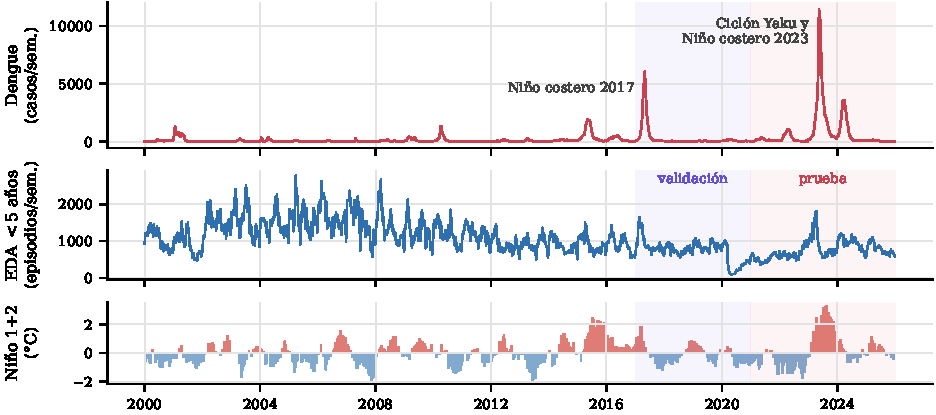
\includegraphics[width=\textwidth]{fig_series}
\caption{Casos semanales en las 14 provincias de la costa norte y anomalía Niño 1+2 (con el rezago de un mes que usa el modelo). Las franjas marcan los periodos de validación (2017--2020) y prueba (2021--2025).}\label{fig:series}
\end{figure*}

% =====================================================================
\section{Metodología}
\subsection{Planteamiento del problema}
Sea $c_{p,t}$ el número de casos de la provincia $p$ en la semana $t$ y $y_{p,t}=\log(1+c_{p,t})$. Al cierre de la semana $t$, el modelo recibe una ventana $\mathbf{X}_{p,t}\in\mathbb{R}^{L\times F}$ con las últimas $L=26$ semanas de $F=10$ variables (casos en logaritmo, seno y coseno de la semana del año, temperatura media, máxima y mínima, lluvia en logaritmo, humedad, Niño 1+2 y ONI) y el índice de la provincia, y devuelve $\hat{y}_{p,t+h}$ para $h=1,\dots,8$. Un horizonte de 8 semanas cubre el tiempo de entrega de un pedido (4 semanas) con margen. Se entrena un modelo para dengue y otro para EDA, compartido por las 14 provincias.

\subsection{Arquitecturas}
Las tres redes comparten la misma estructura (Fig.~\ref{fig:arq}): un codificador lee la ventana, una capa lineal produce los 8 horizontes a la vez y una conexión residual suma el último valor observado, $\hat{y}_{t+h}=y_t+f_\theta(\mathbf{X})_h$. Así la red aprende cuánto va a cambiar la serie y no su nivel, que varía en tres órdenes de magnitud entre provincias. La identidad de la provincia entra como un \textit{embedding} aprendido. La LSTM y la GRU tienen 2 capas de 64 unidades con \textit{dropout} de 0,2; el \textit{Transformer} proyecta cada semana a $d=64$, suma una codificación posicional aprendida y aplica 2 capas de codificador con 4 cabezas de atención y normalización previa. Los tamaños son \nPLS{} (LSTM), \nPGR{} (GRU) y \nPTr{} (\textit{Transformer}) parámetros.

\begin{figure}[t]
\centering
\begin{tikzpicture}[font=\scriptsize, node distance=2.5mm and 3.5mm,
  caja/.style={draw, rounded corners=2pt, align=center, inner sep=2.5pt, fill=#1!10},
  caja/.default=gray, flecha/.style={-{Stealth[length=3.5pt]}, semithick}]
\node[caja=blue, text width=1.75cm] (x) {Ventana de 26 sem.: casos, estación, clima, El Niño};
\node[caja=blue, below=of x, text width=1.75cm] (p) {Provincia $p$ (\textit{embedding})};
\node[caja=green, right=4mm of $(x.east)!0.5!(p.east)$, text width=1.95cm] (enc) {\textbf{Codificador}\\[1pt] LSTM o GRU\\ (2 capas, 64)\\[1pt] o \textit{Transformer}\\ ($d$=64, 4 cabezas,\\ 2 capas)};
\node[caja=orange, right=3.5mm of enc, text width=0.95cm] (lin) {Capa lineal\\ 8 salidas};
\node[draw, circle, inner sep=0.8pt, right=2.5mm of lin] (suma) {$+$};
\node[caja=red, right=2.5mm of suma] (y) {$\hat{y}_{t+1}$\\ $\vdots$\\ $\hat{y}_{t+8}$};
\node[caja, below=4mm of $(lin.south)!0.5!(y.south)$, text width=2.6cm] (inv) {Política de stock base: pedido de cada semana};
\draw[flecha] (x.east) -- (x.east -| enc.west);
\draw[flecha] (p.east) -- (p.east -| enc.west);
\draw[flecha] (enc) -- (lin);
\draw[flecha] (lin) -- (suma);
\draw[flecha] (suma) -- (y);
\draw[flecha] (x.north) -- ++(0,3mm) -| (suma.north) node[pos=0.25, above, font=\tiny]{último valor $y_t$ (conexión residual)};
\draw[flecha] (y.south) -- (y.south |- inv.north);
\end{tikzpicture}

\caption{Estructura común de los modelos. La salida en casos, $e^{\hat y}-1$, alimenta la política de pedidos.}\label{fig:arq}
\end{figure}

\subsection{Líneas base}
Comparamos con cuatro referencias: (i) \emph{persistencia}, que repite el último valor observado en los 8 horizontes; (ii) \emph{canal endémico}, la mediana de la misma semana en los 5 años anteriores, que es lo que se usa hoy para planificar; (iii) \emph{ARIMA(2,0,1)} por provincia con 3 pares de términos de Fourier para la estacionalidad anual \cite{hyndman2021fpp3}, reestimado con todos los datos previos al inicio de cada periodo; y (iv) un \emph{random forest} \cite{breiman2001rf} de 200 árboles con la ventana aplanada y el mismo objetivo residual que las redes.

\subsection{Partición, entrenamiento y métricas}
Usamos una partición temporal: entrenamiento 2000--2016, validación 2017--2020 y prueba 2021--2025. Se descartan las ventanas cuya historia o cuyo horizonte cruzan de un periodo a otro, de modo que ninguna semana del periodo de prueba se ve durante el entrenamiento ni durante la selección del modelo; las medias y desviaciones para estandarizar se calculan solo con el entrenamiento. Esto deja \nnTr{} ventanas para entrenar, \nnVa{} para validar y \nnTe{} para probar. Cada red se entrena con error cuadrático medio en escala logarítmica, AdamW \cite{loshchilov2019adamw} (tasa 0,001, lote 256) y parada temprana con paciencia de 8 épocas sobre la pérdida de validación, repitiendo todo con cinco semillas (0 a 4).

Reportamos el error absoluto medio (MAE) y la raíz del error cuadrático medio (RMSE) en casos por provincia y semana, promediados sobre los 8 horizontes; el MAE en escala logarítmica, que pesa por igual a provincias grandes y pequeñas; el MAE en validación, que es el criterio con el que se elegiría un modelo; y el F1 de una alerta: con 4 semanas de anticipación, ¿superará la semana el percentil 90 de los 5 años previos de esa provincia?

\subsection{Interpretabilidad}
Para saber en qué se fija la red usamos gradientes integrados \cite{sundararajan2017ig} sobre la LSTM de menor pérdida de validación, con 32 pasos, la ventana en cero (es decir, en la media del entrenamiento) como referencia y la salida a 4 semanas como objetivo. Promediamos el valor absoluto de las atribuciones en 1\,000 ventanas de prueba y las agrupamos en historia de casos, estacionalidad, clima y El Niño.

\subsection{Del pronóstico al pedido}
Cada semana $t$ y en cada provincia, el responsable de farmacia pide lo necesario para que el inventario disponible más lo que está en camino alcance el nivel objetivo
\begin{equation}
S_t=\sum_{h=1}^{\ell}\hat{D}_{t+h}+z\,\sigma_\ell ,\label{eq:stock}
\end{equation}
donde $\hat{D}_{t+h}$ es la demanda pronosticada en tratamientos (un tratamiento por caso), $\ell=4$ semanas es el tiempo de entrega, $z=1{,}65$ corresponde a un nivel de servicio objetivo de 95\,\% y $\sigma_\ell$ es la desviación del error del pronóstico acumulado de 4 semanas en el periodo de validación \cite{silver2017inventory}. Lo que no se puede atender en la semana se pierde. Simulamos 2021--2025 con cuatro fuentes de pronóstico: canal endémico, \textit{random forest}, LSTM y un pronóstico perfecto como cota. El paso de tratamientos a unidades de cada medicamento usa un kit por grupo clínico (Tabla~\ref{tab:fuentes}) que el usuario puede editar.

% =====================================================================
\section{Resultados}
\subsection{Dengue}
La Tabla~\ref{tab:dengue} resume la comparación. Las tres redes y el \textit{random forest} superan a todas las líneas base clásicas. El \textit{Transformer} obtiene el menor error en validación y en prueba (MAE de \nDTrMAE{} casos frente a \nDPersMAE{} de la persistencia y \nDArimaMAE{} de ARIMA), aunque el \textit{random forest} queda prácticamente empatado (\nDRFMAE) y la diferencia entre redes es menor que la variación entre semillas. El canal endémico es, con diferencia, la peor referencia: al usar la mediana de años pasados no anticipa ningún brote, de ahí su F1 cercano a cero. La persistencia, en cambio, tiene un F1 alto (\nDPersFUno), porque un brote que ya empezó suele seguir por encima del umbral cuatro semanas después; todos los modelos que ven los casos recientes quedan en ese mismo nivel.

\begin{table}[t]
\centering\caption{Dengue: error en prueba (2021-2025) y en validación (2017-2020). Media $\pm$ d.e. de 5 semillas; MAE y RMSE en casos por provincia y semana, promedio de los 8 horizontes; F1 de alerta a 4 semanas.}\label{tab:dengue}
\setlength{\tabcolsep}{2.3pt}\footnotesize
\begin{tabular}{lccccc}
\toprule
Modelo & MAE val. & MAE & RMSE & MAE log & F1 \\
\midrule
Persistencia & 17.1 & 38.5 & 171.7 & 0.647 & 0.807 \\
Canal endémico & 25.3 & 56.0 & 218.1 & 1.634 & 0.008 \\
ARIMA + Fourier & 12.7 & 34.5 & 161.6 & 0.646 & 0.757 \\
Random forest & 11.3 & 29.9{\tiny$\,\pm$0.2} & 149.3{\tiny$\,\pm$0.7} & 0.612{\tiny$\,\pm$0.001} & 0.803{\tiny$\,\pm$0.003} \\
\midrule
LSTM & 11.1{\tiny$\,\pm$0.8} & 31.8{\tiny$\,\pm$0.8} & 157.0{\tiny$\,\pm$6.5} & \textbf{0.605{\tiny$\,\pm$0.011}} & \textbf{0.809{\tiny$\,\pm$0.007}} \\
GRU & 11.1{\tiny$\,\pm$0.5} & 31.7{\tiny$\,\pm$0.9} & 151.9{\tiny$\,\pm$4.9} & 0.619{\tiny$\,\pm$0.012} & 0.806{\tiny$\,\pm$0.007} \\
Transformer & \textbf{10.9{\tiny$\,\pm$0.5}} & \textbf{29.8{\tiny$\,\pm$0.9}} & \textbf{147.8{\tiny$\,\pm$5.0}} & 0.607{\tiny$\,\pm$0.022} & 0.808{\tiny$\,\pm$0.008} \\
\bottomrule
\end{tabular}
\end{table}


La ventaja de las redes crece con el horizonte (Fig.~\ref{fig:horizonte}). A una semana, la persistencia (\nHUnoPers) y el \textit{random forest} (\nHUnoRF) son tan buenos como cualquier red, lo cual es esperable: la serie casi no cambia de una semana a otra. A 8 semanas, en cambio, el error del \textit{Transformer} (\nHOchoTr) es \nredHochoTrPers\,\% menor que el de la persistencia (\nHOchoPers) y \nredHochoTrArima\,\% menor que el de ARIMA (\nHOchoArima). Ese tramo es justamente el que importa para pedir medicamentos con cuatro semanas de anticipación.

\begin{figure}[t]
\centering
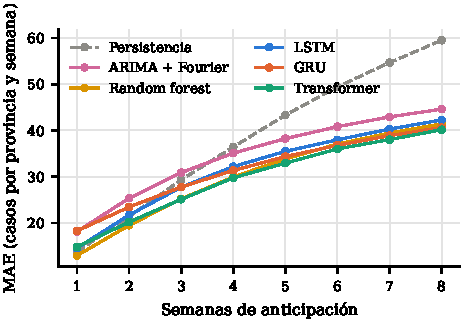
\includegraphics[width=\columnwidth]{fig_horizonte}
\caption{Dengue: MAE en el periodo de prueba según las semanas de anticipación (media de 5 semillas).}\label{fig:horizonte}
\end{figure}

El RMSE es mucho mayor que el MAE porque los errores se concentran en pocas semanas. En las semanas en que la provincia estaba en alerta (\npctAlerta\,\% del periodo de prueba), el error a 4 semanas del \textit{Transformer} sube a \nAlTrAlerta{} casos, frente a \nAlTrNormal{} en semanas normales. El caso más difícil es Piura en 2023 (Fig.~\ref{fig:piura}): en la semana de mayor transmisión hubo \npicoReal{} casos y el \textit{Transformer}, con cuatro semanas de anticipación, pronosticó \npicoTr. Las redes reaccionan antes y con más fuerza que ARIMA, pero ninguna anticipa la magnitud del pico, que no tiene precedente en el entrenamiento.

\begin{figure}[t]
\centering
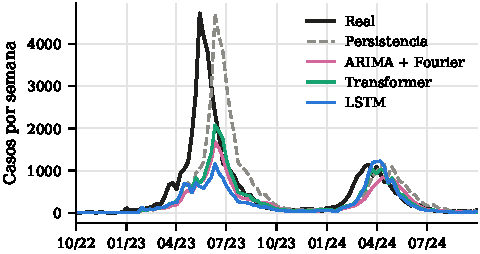
\includegraphics[width=\columnwidth]{fig_piura}
\caption{Piura, octubre de 2022 a setiembre de 2024 (periodo de prueba): casos observados y pronóstico hecho 4 semanas antes.}\label{fig:piura}
\end{figure}

\subsection{EDA en menores de 5 años}
La EDA en menores de 5 años es una serie mucho más regular y las diferencias entre modelos son pequeñas (Tabla~\ref{tab:eda}). La GRU obtiene el menor MAE de prueba (\nEGRUMAE{} episodios por provincia y semana) y el menor RMSE (\nEGRURMSE), con una mejora de \nredEPers\,\% sobre la persistencia y de \nredEArima\,\% sobre ARIMA, pero queda prácticamente empatada con el \textit{random forest} (\nERFMAE), que además tiene el menor error en validación y en escala logarítmica. Como en el dengue, la ventaja de las redes aparece en los horizontes largos: a una semana todos los modelos rondan los 10 episodios, mientras que a 8 semanas el \textit{Transformer} (\nEHOchoTr) reduce en \nredEHochoTrPers\,\% el error de la persistencia (\nEHOchoPers). El F1 es más bajo que en el dengue (cerca de 0,5) porque las semanas de alerta de EDA son subidas cortas sobre una estacionalidad estable; en esta tarea ARIMA, que modela mejor esa estacionalidad, es el que mejor anticipa las alertas.


\begin{table}[t]
\centering\caption{EDA en menores de 5 años: mismas métricas que la Tabla~\ref{tab:dengue}.}\label{tab:eda}
\setlength{\tabcolsep}{2.3pt}\footnotesize
\begin{tabular}{lccccc}
\toprule
Modelo & MAE val. & MAE & RMSE & MAE log & F1 \\
\midrule
Persistencia & 15.8 & 14.3 & 27.9 & 0.338 & 0.496 \\
Canal endémico & 21.7 & 20.9 & 38.3 & 0.460 & 0.014 \\
ARIMA + Fourier & 15.2 & 14.7 & 27.1 & 0.310 & \textbf{0.534} \\
Random forest & \textbf{14.2} & 13.6 & 27.0 & \textbf{0.305} & 0.509{\tiny$\,\pm$0.003} \\
\midrule
LSTM & 15.5{\tiny$\,\pm$0.2} & 14.0{\tiny$\,\pm$0.3} & 26.0{\tiny$\,\pm$0.7} & 0.331{\tiny$\,\pm$0.005} & 0.489{\tiny$\,\pm$0.010} \\
GRU & 15.2{\tiny$\,\pm$0.1} & \textbf{13.5{\tiny$\,\pm$0.3}} & \textbf{24.8{\tiny$\,\pm$0.8}} & 0.322{\tiny$\,\pm$0.005} & 0.487{\tiny$\,\pm$0.012} \\
Transformer & 14.9{\tiny$\,\pm$0.4} & 13.8{\tiny$\,\pm$0.5} & 25.4{\tiny$\,\pm$0.5} & 0.318{\tiny$\,\pm$0.011} & 0.476{\tiny$\,\pm$0.032} \\
\bottomrule
\end{tabular}
\end{table}


\subsection{Ablación}
La Tabla~\ref{tab:ablacion} repite el entrenamiento de la LSTM quitando un componente a la vez. Quitar la conexión residual es lo que más daño hace: el MAE de prueba sube de \nAbcompletoMAE{} a \nAbsinresidualMAE{} casos, peor incluso que ARIMA. Quitar el clima empeora el error de validación (de \nAbcompletoMAEval{} a \nAbsinclimaMAEval) y el RMSE, pero en el periodo de prueba el modelo sin clima, sin El Niño o solo con casos y estacionalidad queda igual o ligeramente mejor (por ejemplo, \nAbsolocasosMAE{} con solo casos), con diferencias del orden de una o dos desviaciones entre semillas. Nuestra lectura es que, a escala de provincia y semana, la información útil del clima ya está en buena parte contenida en la estación y en los casos recientes, y que la relación clima--dengue aprendida antes de 2017 no se trasladó bien a 2023, cuando la lluvia extrema del ciclón Yaku y la respuesta sanitaria cambiaron la dinámica.

\begin{table}[t]\centering\caption{Ablación de la LSTM para dengue (5 semillas, misma partición). El modelo completo usa casos, estacionalidad, clima y El Niño con conexión residual.}\label{tab:ablacion}
\setlength{\tabcolsep}{3pt}\footnotesize\begin{tabular}{lcccc}\toprule
Variante & MAE val. & MAE & RMSE & F1 \\\midrule
Completo & 11.1{\tiny$\,\pm$0.8} & 31.8{\tiny$\,\pm$0.8} & 157.0{\tiny$\,\pm$6.5} & 0.809 \\
Sin clima & 11.7{\tiny$\,\pm$0.6} & 32.0{\tiny$\,\pm$0.9} & 161.6{\tiny$\,\pm$5.0} & 0.819 \\
Sin El Niño & 11.1{\tiny$\,\pm$0.6} & 30.5{\tiny$\,\pm$1.2} & 146.6{\tiny$\,\pm$8.8} & 0.808 \\
Solo casos y estación & 11.2{\tiny$\,\pm$0.4} & 30.4{\tiny$\,\pm$0.6} & 153.5{\tiny$\,\pm$2.1} & 0.826 \\
Sin conexión residual & 14.6{\tiny$\,\pm$0.8} & 40.4{\tiny$\,\pm$1.1} & 192.3{\tiny$\,\pm$4.2} & 0.739 \\
\bottomrule\end{tabular}\end{table}


\subsection{Interpretabilidad}
Los gradientes integrados confirman esa lectura (Fig.~\ref{fig:ig}). La historia de casos concentra el \nIGHist\,\% de la atribución, la estacionalidad el \nIGEst\,\%, el clima el \nIGClima\,\% y El Niño apenas el \nIGNino\,\%. Dentro de la ventana, la red se apoya sobre todo en las últimas 4 a 6 semanas de casos; las variables de clima reciben atribución más repartida a lo largo de la ventana, compatible con los rezagos de varias semanas que describe la literatura entomológica \cite{morin2013climate}.

\begin{figure}[t]
\centering
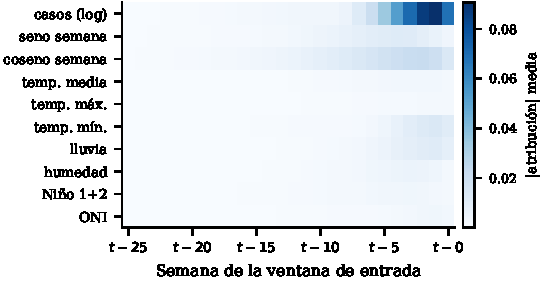
\includegraphics[width=\columnwidth]{fig_ig}
\caption{Gradientes integrados de la LSTM (salida a 4 semanas): atribución absoluta media por variable y semana de la ventana, en 1\,000 ventanas de prueba.}\label{fig:ig}
\end{figure}

\subsection{Abastecimiento}
La Tabla~\ref{tab:stock} y la Fig.~\ref{fig:stock} muestran el efecto en el inventario. Planificar con el canal endémico deja sin atender \nSCanalfal{} tratamientos en cinco años y alcanza un nivel de servicio de solo \nSCanalns\,\%, aun manteniendo el doble de inventario: acumula stock en los años tranquilos y se queda corto cuando llega el brote. Con el pronóstico de la LSTM el nivel de servicio sube a \nSLSTMns\,\%, los tratamientos no atendidos bajan \nredSfal\,\% y el inventario promedio baja \nredSinv\,\%. El \textit{random forest} logra un resultado parecido (\nSRFns\,\%). La distancia con el pronóstico perfecto se explica por los picos de 2023 y por un tiempo de entrega de 4 semanas que no deja corregir a tiempo.

\begin{table}[t]\centering\caption{Simulación de stock base para dengue en las 14 provincias, 2021-2025 (tiempo de entrega de 4 semanas, $z=1{,}65$). Inventario en tratamientos al cierre de cada semana.}\label{tab:stock}
\setlength{\tabcolsep}{3pt}\footnotesize\begin{tabular}{lcccc}\toprule
Política & \begin{tabular}[c]{@{}c@{}}Nivel de\\servicio (\%)\end{tabular} & \begin{tabular}[c]{@{}c@{}}No\\atendidos\end{tabular} & \begin{tabular}[c]{@{}c@{}}Semanas con\\quiebre (\%)\end{tabular} & \begin{tabular}[c]{@{}c@{}}Inventario\\promedio\end{tabular} \\\midrule
Canal endémico & 44.9 & 107\,468 & 26.0 & 5\,340 \\
Random forest & 75.3 & 48\,111 & 14.8 & 2\,740 \\
LSTM & 71.9 & 54\,787 & 14.4 & 2\,897 \\
Pronóstico perfecto & 100.0 & 0 & 0.0 & 1 \\
\bottomrule\end{tabular}\end{table}


\begin{figure}[t]
\centering
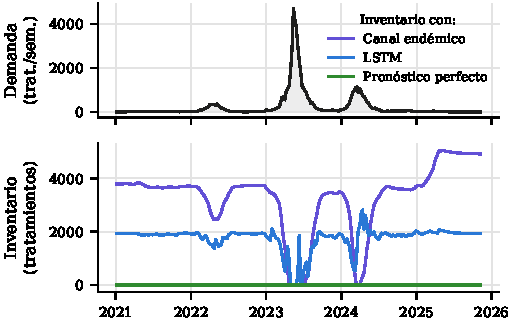
\includegraphics[width=\columnwidth]{fig_stock}
\caption{Piura, 2021--2025: demanda semanal de tratamientos para dengue e inventario simulado al cierre de cada semana con tres fuentes de pronóstico.}\label{fig:stock}
\end{figure}

\subsection{Costo computacional}
Todo se entrenó en una CPU Intel Xeon de 2 núcleos a 2,1~GHz con 8~GB de RAM, sin GPU, con PyTorch (Tabla~\ref{tab:costo}). Las 30 redes de la comparación principal (3 arquitecturas, 5 semillas, 2 enfermedades) tomaron \nminRedes{} minutos y el proyecto completo, con líneas base, ablaciones e interpretabilidad, unos \nminNotebook{} minutos, de modo que puede reproducirse en Google Colab sin GPU. La inferencia es trivial: el aplicativo ejecuta las 15 redes de una enfermedad para las 14 provincias en menos de un segundo dentro del navegador, con los pesos guardados en media precisión (diferencia máxima de $5\times10^{-4}$ en escala logarítmica respecto a PyTorch).

\begin{table}[t]\centering\caption{Tamaño y costo de entrenamiento por semilla (CPU de 2 núcleos, sin GPU). Los tiempos varían con la carga de la máquina.}\label{tab:costo}
\setlength{\tabcolsep}{4pt}\footnotesize\begin{tabular}{lcccc}\toprule
Modelo & Parámetros & Épocas & \begin{tabular}[c]{@{}c@{}}Segundos\\(dengue)\end{tabular} & \begin{tabular}[c]{@{}c@{}}Segundos\\(EDA)\end{tabular} \\\midrule
LSTM & 54\,336 & 10.8 & 54 & 14 \\
GRU & 40\,896 & 14.8 & 31 & 21 \\
Transformer & 70\,856 & 11.4 & 51 & 64 \\
\bottomrule\end{tabular}\end{table}


% =====================================================================
\section{Discusión}
\subsection{Herramienta para pronosticar}
Para que el modelo sirva fuera del cuaderno de trabajo, construimos un aplicativo web de un solo archivo que reproduce en JavaScript el cálculo de las tres redes. El usuario elige la enfermedad, la provincia, el modelo y un horizonte de 1 a 26 semanas desde la última semana con datos o desde cualquier fecha pasada (para comparar con lo que realmente ocurrió). Puede plantear escenarios (más calor, más lluvia, Niño costero moderado o fuerte, año frío), corregir los casos de las últimas semanas si tiene datos más recientes que el archivo abierto, y guardar cada pronóstico para compararlo semana a semana con otros. Hasta 8 semanas el pronóstico es directo; más allá se encadena usando el clima normal de cada semana (2000--2020) ajustado por el escenario, y la banda del 80\,\% se ensancha con la raíz del horizonte. Además, el usuario puede \emph{avanzar en el tiempo}: el pronóstico de las 14 provincias se agrega al historial como si esas semanas ya hubieran ocurrido y el modelo vuelve a pronosticar desde ahí, de una en una, de cuatro en cuatro o en forma automática, con la posibilidad de cambiar el escenario o escribir un brote en cualquier paso y de deshacerlo. Así se puede ensayar cómo evolucionaría una temporada y cuánto habría que pedir en cada semana. Un botón calcula el mismo pronóstico con los seis escenarios predefinidos y los compara en una tabla y un gráfico. El aplicativo también traduce el pronóstico de las 14 provincias en un pedido sugerido de cada medicamento a partir del stock y de lo que está en camino; allí el stock de seguridad se calcula con los cuantiles del error de validación en escala logarítmica, de modo que crece con el nivel pronosticado en lugar de ser fijo.

\subsection{Limitaciones}
Primero, los datos de vigilancia cuentan casos notificados, no infecciones; el subregistro varía entre provincias y en el tiempo, y los últimos meses siempre están incompletos. Segundo, el periodo de prueba está dominado por un evento extremo (2023): los errores grandes se concentran ahí y las conclusiones sobre el clima podrían cambiar con más años. Tercero, el clima es el de un punto por provincia y no captura la heterogeneidad dentro de ella. Cuarto, el kit de medicamentos por caso y el tiempo de entrega son supuestos razonables que deben validarse con las direcciones regionales de salud. Por último, más allá de 8 semanas el aplicativo no pronostica el clima: lo supone igual al normal más el escenario que elige el usuario, y así debe leerse.

\subsection{Uso responsable}
Los datos son agregados por provincia y semana, públicos y sin información personal; respetamos la licencia ODC-By citando la fuente. El modelo no reemplaza a la vigilancia epidemiológica ni al juicio de quien decide: subestima los picos sin precedente, y una lectura literal en un año como 2023 llevaría a pedir menos de lo necesario. Por eso el aplicativo muestra siempre la banda de incertidumbre, el error histórico por horizonte y el canal endémico como referencia. También existe el riesgo contrario, el de sobrerreaccionar a un escenario extremo planteado por el usuario; el aplicativo deja claro qué parte del pronóstico depende de supuestos.

% =====================================================================
\section{Conclusiones}
Con datos abiertos es posible pronosticar el dengue y la EDA infantil en la costa norte del Perú con varias semanas de anticipación y con un error claramente menor al de las herramientas que se usan hoy. Las redes neuronales aportan sobre todo en los horizontes largos, que son los que permiten actuar, y su valor se ve mejor cuando se mide en tratamientos atendidos que en errores promedio. El componente decisivo fue la conexión residual y no la cantidad de variables: el clima aporta poco una vez que la red conoce los casos recientes y la estación, y El Niño, usado sin adelantarse a su publicación, casi nada. Como trabajo futuro planteamos incorporar pronósticos climáticos estacionales en lugar del clima normal, pronósticos probabilísticos entrenados con pérdida de cuantiles, datos de más regiones y la validación del kit de medicamentos con las redes de salud.

% =====================================================================
\section*{Contribuciones del equipo}
\begin{table}[h]
\centering
\caption{Contribución de cada integrante.}\label{tab:contrib}
\setlength{\tabcolsep}{3pt}\footnotesize
\begin{tabular}{>{\raggedright\arraybackslash}p{2.5cm}>{\raggedright\arraybackslash}p{5.4cm}}
\toprule
Integrante & Contribución \\
\midrule
Fernando Tapia Álvarez & Descarga y limpieza de los datos del CDC y de NASA POWER; construcción del panel y del Excel. \\
Ana Rocio Cuchuirumi Merma & Análisis exploratorio, validación contra boletines y líneas base (canal endémico y ARIMA). \\
Edgard Antonio Quispe Arias & Implementación y entrenamiento de LSTM, GRU y \textit{Transformer}; ablaciones. \\
Matías Samuel Ochoa Alejos & Simulación de abastecimiento, kit de medicamentos y aplicativo web. \\
Carlos Cassano Vilca & Interpretabilidad, redacción del artículo y repositorio. \\
\bottomrule
\end{tabular}
\end{table}
Todos los integrantes revisaron el artículo y aprueban la versión final.

\section*{Disponibilidad de datos y código}
El panel, el código, los cuadernos de Colab, los pesos entrenados y el aplicativo están en \repo{} (versión \texttt{v1.0-final}).

\bibliographystyle{IEEEtran}
\bibliography{referencias}

\end{document}
